%----------------------------------------------------------------------------------------
%	ABSTRACT
%----------------------------------------------------------------------------------------

% The first character should be within \initial{}
\initial{Ο}{\color{teal}ι κανονικές εκφράσεις είναι ένας πανίσχυρος μηχανισμός που μας επιτρέπει να ψάχνουμε για συγκεκριμένα πρότυπα (patterns) σε κείμενα. Χρησιμοποιείται σαν όρισμα σε αρκετές εντολές του UNIX αλλά και σχεδόν σε όλες τις γλώσσες προγραμματισμού.}

%----------------------------------------------------------------------------------------
%	ARTICLE CONTENTS
%----------------------------------------------------------------------------------------



%------------------------------------------------


\epigraphhead[10]{\epigraph{"Contrary to popular belief, Unix is user friendly. It just happens to be very selective about who it decides to make friends with. "}{\textit{\href{}{}}}}

\section{Console Editors}
Οι πιο δημοφιλής editors στο UNIX είναι οι παρακάτω:
\begin{itemize}
	\item vi / vim \cite{Neil:2015}. Υπάρχει σε κάθε UNIX σύστημα. Δείτε το \href{https://www.cs.colostate.edu/helpdocs/vi.html}{manual}
	\item nano / pico. Εύχρηστος, απλός editor. Δείτε το \href{http://documentation.its.umich.edu/node/241}{manual}
	\item emacs. Παλαιότερος όλων. Διαφέρει αρκετά από τους άλλους editors.
\end{itemize}

Για να μπορέσετε να χρησιμοποιήσετε τους console editors χρειαζεται να έχει οριστεί το terminal emulation package και το πιο δημοφιλές είναι το xterm. Σε περίπτωση που δεν σας λειτουργεί (Unknown terminal type error) ο editor δοκιμάστε την εξής εντολή \texttt{export TERM=xterm}. Περισσότερα για τη μεταβλητή TERM  \href{http://jdebp.eu./Softwares/nosh/guide/TERM.html}{εδώ}.

\begin{tcolorbox}[frogbox, title=vifm]
	Αν ενδιαφέρεστε για έναν treminal file manager με επιρροές από τον vim editor, δοκιμάστε τον vifm. Δείτε τον  \href{https://wiki.vifm.info/index.php/Quickstart_Tutorial}{οδηγό χρήσης του vifm}.
\end{tcolorbox}


\section{Κανονικές εκφράσεις}



Είδαμε ότι με την εντολή grep μπορούμε να  κάνουμε αναζήτηση σχηματισμών σε αρχεία. Μπορούμε να χρησιμοποιήσουμε πιο πολύπλοκες εκφράσεις
για αναζήτηση, οι οποίες ονομάζονται \textbf{κανονικές εκφράσεις} (regular expressions ή regex) \cite{nemeth2011unix}\cite{kochan2016shell}. Οι κανονικές εκφράσεις είναι ένας
μηχανισμός ταιριάσματος προτύπων. Αντίθετα με το μηχανισμό που χρησιμοποιεί ο φλοιός για τη δημιουργία ονομάτων αρχείων, οι κανονικές
εκφράσεις προσφέρουν κυρίως ισχύ και όχι ευκολία χρήσης. Ωστόσο, με την εξάσκηση και προσεκτική επισκόπηση όσων κανονικών εκφράσεων
συναντάτε, μπορείτε να εκμεταλλευτείτε αυτό το δυνατό εργαλείο. Ανάμεσα στα πολλά utilities που τα χρησιμοποιούν, είναι οι: grep, sed, less, vi και awk.

Οι κανονικές εκφράσεις χρησιμοποιούνται για να φιλτράρουμε κάποιο κείμενο \cite{blum2008linux}. Αποτελούν όρισμα σε αρκετές εντολές και γλώσσες προγραμματισμού και είναι ένας πανίσχυρος μηχανισμός ταιριάσματος προτύπων. Η λογική με την οποία λειτουργούν είναι απλή και φαίνεται στην εικόνα \ref{fig:reg-ex}.
Υπάρχουν δυο εκδοχές των κανονικών εκφράσεων στο UNIX:
\begin{itemize}
	\item \textbf{Basic Regular Expressions (BRE)}. Υποστηρίζονται από αρκετές εντολές του UNIX. Κάποιες ωστόσο υποστηρίζουν ακόμη και ένα υποσύνολο των BRE. Σε κάθε περίπτωση πρέπει να βλέπετε το manual των εντολών.
	\item \textbf{Extended Regular Expressions (ERE)}. Συνήθως υποστηρίζεται στις γλώσσες προγραμματισμού. Υποστηρίζουν περισσότερα σύμβολα και λειτουργίες. Κάποιες εντολές υποστηρίζουν τις ERE όταν βάλουμε κάποιο συγκεκριμένη παράμετρο (option).
\end{itemize}

\begin{figure}
	\centering
	\scalebox{0.3}{\includegraphics{images/reg-ex.png}}
	\caption{Η λογική των κανονικών εκφράσεων}
	\label{fig:reg-ex}
\end{figure} 

Υπάρχουν δυο ειδών regular expressions: τα βασικά και τα extended. Κάποια προγράμματα χρησιμοποιούν τα βασικά, όπως ο vi, sed, grep, more και άλλα τα extended, όπως το awk, egrep.

Οι κανονικές εκφράσεις μπορούν να χωριστούν σε τρεις κατηγορίες:
\begin{packed_item}
	\item \textbf{wildcards}, χρησιμοποιούνται στη θέση κάποιου άλλου χαρακτήρα
	\item \textbf{modifiers}, χρησιμοποιούνται για να τροποποιήσουν τον προηγούμενο χαρακτήρα
	\item \textbf{anchors}, χρησιμοποιούνται για να «αγκιστρώσουν» μία συμβολοσειρά στην αρχή ή στο τέλος μίας γραμμής ή λέξης
\end{packed_item}

\subsection{wildcards - quotations}

Κάποιοι χαρακτήρες είναι ειδικοί χαρακτήρες όταν χρησιμοποιούνται σε κανονικές εκφράσεις. Αυτοί είναι οι:
\begin{lstlisting}
. * [] {} ^ \$ \ + ? | ()
\end{lstlisting}


Μερικές φορές θέλουμε να αναφερθούμε σε πολλά αρχεία με ένα πέρασμα. Για παράδειγμα αν θέλουμε να αντιγράψουμε όλα τα αρχεία που έχουν
κατάληξη .c σε ένα άλλο φάκελο, θα χρησιμοποιήσουμε wildcards. Είναι κάποιοι χαρακτήρες σαν το * και το ?, οι οποίοι αναπαριστούν
οποιονδήποτε ή ένα σύνολο από χαρακτήρες. Είναι κάτι σαν τον μπαλαντέρ στα χαρτιά. Τα σύμβολα που μπορούν να είναι wildcards παρουσιάζονται
στον πίνακα \ref{wildcards}.

\begin{table}[h]
	\begin{tabularx}{\columnwidth}{r|X}
		.   & ταιριάζει οποιονδήποτε χαρακτήρα εκτός από το newline \\
		? 	& ταιριάζει έναν οποιονδήποτε χαρακτήρα. Προσοχή: Υποστηρίζεται μόνο στις Extended Regular Expressions. Για να χρησιμοποιηθεί σε κάποιες εντολές όπως η grep θα πρέπει να χρησιμοποιήσουμε κάποια παράμετρο (-E στην grep)\\
		* 	& ταιριάζει 0 ή περισσότερους χαρακτήρες, εκτός αν ο αρχικός είναι η τελεία\\
		$[C_{1}C_{2}$ ... $C_{n}]$ 	& Αναφέρεται σε οποινδήποτε χαρακτήρα που εμπεριέχεται στη λίστα (character class) \\			
		$[C_{1}$ - $C_{n}]$ 		& Αναφέρεται σε οποινδήποτε χαρακτήρα που εμπεριέχεται στη λίστα, \\
		& η λίστα ξεκινάει από τον πρώτο χαρακτήρα μέχρι τον τελευταίο $[C_{1}$ -$C_{n}]$.\\
		$[  \hat{ }abc]$ & Αναφέρεται σε οποινδήποτε χαρακτήρα που δεν εμπεριέχεται στη λίστα\\
		" " & «άπλωσε» τις εντολές και τις μεταβλητές \\
		' ' & παρέθεσε ακριβώς την έκφραση \\
		$\backslash$ & παρέθεσε ακριβώς τον επόμενο χαρακτήρα \\
	\end{tabularx}  
	
	\caption{Wildcards και quotations}
	\label{wildcards}
\end{table}


\subsubsection{Special Character Classes}
Στις κανονικές εκφράσεις υπάρχουν και κάποιες συγκεκριμένες character classes τις οποίες μπορούμε να χρησιμοποιούμε \footnote{Στο Solaris η grep παίρνει σαν όρισμα κανονικές εκφράσεις. Προσοχή όμως γιατί η /usr/bin/grep δέχεται μόνο ένα υποσύνολο των κανονικών εκφράσεων. Αν θέλουμε να χρησιμοποιήσουμε τα special character classes θα πρέπει να χρησιμοποιήσουμε την /usr/xpg4/bin/grep βάζοντας και την παράμετρο -E. Στο Linux η grep τα υποστηρίζει κανονικά.}. Αυτές οι κλάσεις\footnote{Πηγή \href{http://www.petefreitag.com/cheatsheets/regex/character-classes/}{https://goo.gl/ncAEBm}}  φαίνονται στον Πίνακα \ref{tbl:re-classes}. 


	

\begin{table}[h]
	\begin{tabularx}{\columnwidth}{l|X}
		\textbf{[:alnum:]} & Αλφαριθμητικοί χαρακτήρες. Περιλαμβάνει γράμματα και αριθμούς. Δεν περιλαμβάνει τα σημεία στίξης \\
		\textbf{[:alpha:]} & Περιλαμβάνει μόνο τα γράμματα\\
		\textbf{[:blank:]} & Χαρακτήρες όπως το κενό και το tab\\
		\textbf{[:cntrl:]} & Χαρακτήρες control (μη εκτυπώσιμοι)\\	
		\textbf{[:digit:]} & Αριθμοί από 0-9\\
		\textbf{[:graph:]} & Τα [:punct:], [:upper:], [:lower:], [:digit:] μαζί \\
		\textbf{[:lower:]} & Οποιοσδήποτε πεζός αλφαβητικός χαρακτήρας \\
		\textbf{[:print:]} & Οποιοσδήποτε εκτυπώσιμος χαρακτήρας\\	
		\textbf{[:punct:]} & Οποιοσδήποτε χαρακτήρας στίξης \\
		\textbf{[:space:]} & Οποιοσδήποτε white space χαρακτήρας: space, Tab, NL, FF, VT, CR \\
		\textbf{[:upper:]} &  Οποιοσδήποτε κεφαλαίος αλφαβητικός χαρακτήρας\\
		\textbf{[:xdigit:]} & Οποιοδήποτε χαρακτήρας του δεκαεξαδικού\\			
	\end{tabularx}  
	\caption{RE character classes}
	\label{tbl:re-classes}
\end{table}



\begin{table}[h]
	\small
	\begin{tabularx}{\columnwidth}{l|X}
		/etc/rc.???? 	& αναφέρεται σε όλα τα αρχεία στο φάκελο /etc τα οποία ξεκινούν από rc.  
		και το όνομά τους έχει μέγεθος 7 χαρακτήρων \\
		*.c  		& Αναφέρεται σε όλα τα αρχεία που έχουν κατάληξη  .c (C προγράμματα)  \\
		*.[Cc] 	& Αναφέρεται σε όλα τα αρχεία που έχουν κατάληξη  .c ή .C  (C ή C++  προγράμματα)  \\
		*.[a-z]  	& Αναφέρεται σε όλα τα αρχεία που έχουν κατάληξη από .a μέχρι .z \\
		
	\end{tabularx}  
	\caption{Παραδείγματα χαρακτήρων μπαλαντέρ}
\end{table}



Είναι σημαντικό να ξέρουμε ότι το κέλυφος «απλώνει» τους χαρακτήρες-μπαλαντέρ: Δηλαδή όταν δίνουμε μια εντολή το πρόγραμμα δεν ξεκινά με μια
παράμετρο που περιέχει χαρακτήρα wildcard, αλλά το κέλυφος «ανοίγει» το wildcard χαρακτήρα πρώτα και μετά εκτελεί την εντολή με τη λίστα των
παραμέτρων που προκύπτουν από την αντικατάσταση των μπαλαντέρ με όλες τις πιθανές τιμές που παίρνουν. 

Για παράδειγμα δοκιμάστε να δημιουργήσετε καταλόγους στον προσωπικό σας φάκελο, της μορφής dir1, dir2, ..., dir9 και μετά να τους
διαγράψετε.

Χρειάζεται ιδιαίτερη προσοχή όταν διαγράφουμε αρχεία και καταλόγους και χρησιμοποιούμε wildcards. Τι θα γίνει αν εκτελέσουμε την εντολή
\texttt{rm *} ; Μην το κάνετε!

\textbf{Προσοχή!} Η αναζήτηση σχηματισμών γίνεται μόνο για τα υπάρχοντα ονόματα αρχείων. Δεν μπορούμε να δημιουργήσουμε νέα ονόματα αρχείων
ή καταλόγων χρησιμοποιώντας σχηματισμούς.\footnote{Για να δημιουργήσουμε νέα αρχεία ή καταλόγους χρησιμοποιούμε τις \{...\}, το οποίο
	σημαίνει «εκτέλεσε τις εντολές που ορίζονται από τα ... ». Για να δημιουργήσουμε καταλόγους π.χ. dir1, ... ,dir9 εκτελούμε την εντολή
	\texttt{mkdir dir\{1..9\}}.}

Ας δημιουργήσουμε κάποιους καταλόγους με δομή κεφαλαίων ενός βιβλίου (chapter1.1, chapter 1.2 ,..., chapter2.1, chapter2.2, ...).Πως θα
γίνει αυτό με μια εντολή;
Τώρα που τους δημιουργήσατε δοκιμάστε να τους μετονομάσετε σε directory1.1 κτλ. Τι παρατηρείτε; 

Το σύμβολο * μπορεί να χρησιμοποιηθεί σε ονόματα διαδρομών. Για παράδειγμα πως θα αναφερθούμε σε όλα τα αρχεια .profile των χρηστών;

%Αν θέλουμε να απενεργοποιήσουμε τη σημασία των χαρακτήρων όπως το *, ? χρησιμοποιούμε είτε '?' είτε \ ? . Δηλαδή αν έχουμε ένα κατάλογο
%?directory θα αναφερθούμε σε αυτόν ως /?directory. 

Μια εξαίρεση: το σύμβολο  .  (τελεία) δεν αντικαθίσταται εάν είναι το πρώτο σύμβολο στο όνομα ενός αρχείου (ή εάν είναι αμέσως μετά απο ένα
/ ).
Δοκιμάστε την ls *. 

Ας υποθέσουμε ότι έχουμε ένα αρχείο το οποίο περιλαμβάνει τα εξής:
\begin{lstlisting}
bt
bat
bet
btt
baat
baaeeet
baeeaeeat
baakeeet
\end{lstlisting}
Δοκιμάστε να βρείτε το pattern \textbf{b[ae]*t} και αιτιολογήστε το αποτέλεσμα.




\subsection{modifiers} 
Ακολουθούν συνήθως ένα χαρακτήρα και τον προσδιορίζουν ποσοτικά. Υποστηρίζονται στις Advanced Regular Expressions.

\begin{packed_item}
	\item \textbf{*} μηδέν ή περισσότεροι από τον προηγούμενο χαρακτήρα
	\item  \textbf{+} ένας ή περισσότεροι από τον προηγούμενο χαρακτήρα
	\item \textbf{?} μηδέν ή ένας από τον ποηγούμενο χαρακτήρα
	\item \textbf{\{i\}} ακριβώς i από τον προηγούμενο χαρακτήρα
	\item \textbf{\{i,\}} i ή περισσότεροι από τον προηγούμενο χαρακτήρα
	\item \textbf{\{i,j\}} i έως j από τον προηγούμενο χαρακτήρα 
\end{packed_item}

Παραδείγματα: \textbf{a*}, \textbf{ab*c}, \textbf{[a-z][a-z][0-9]*}

Οι αγκύλες \{ και \} όταν έπονται του χαρακτήρα \textbackslash (backslash)  συμπεριφέρονται ως μετρητές (counters), και προσδιορίζουν τον
αριθμό του προηγούμενου χαρακτήρα που μας ενδιαφέρει. Παραδείγματα: r\textbackslash\{6\textbackslash\} ,
ca\textbackslash\{5,\textbackslash\}t

\subsubsection{Pipe}

Το σύμβολο (|) μας επιτρέπει να καθορίσουμε δύο ή περισσότερα patterns τα οποία θα ταιριάξει ο μηχανισμός των RE. 
Αν υποθέσουμε ότι έχουμε το αρχείο:
\begin{lstlisting}
Hello there
1 dollar 
there are 3 pets inside
well done
bt
bat
bet
btt
baat
baaeeet
baeeaeeat
baakeeet
\end{lstlisting}

Αν θέλουμε να φέρουμε όλες τις γραμμές οι οποίες περιέχουν λέξεις οι οποίες περιέχουν ένα b το οποίο ακολουθείται από ένα ή περισσότερα a και μετά από ένα t και όλες τις γραμμές οι οποίες περιέχουν αριθμούς, τότε θα εκτελέσουμε την εντολή:



\begin{lstlisting}[upquote=true]
grep -E   "ba{1,}t|[[:digit:]]" file.txt
\end{lstlisting}

όπου file.txt το αρχείο.

\subsubsection{Grouping}
Οι παρενθέσεις χρησιμοποιούνται για να ομαδοποιούμε τις κανονικές εκφράσεις. Όταν ομαδοποιούμε κάτι, αυτό πλέον αντιμετωπίζεται όπως ένας απλός χαρακτήρας.
Παράδειγμα:\\
\begin{lstlisting}
grep -E "b(aee){1,2}" file.txt
\end{lstlisting}



\subsection{anchors} 
Πολλά εργαλεία κειμένου στο UNIX είναι προσανατολισμένα στις γραμμές, δηλαδή κάνουν αναζήτηση για patterns τα οποία περιέχονται μεταξύ δυο
end of line (EOL) seperators. Οι κανονικές εκφράσεις γενικά εξετάζουν το κείμενο το οποίο βρίσκεται ενδιάμεσα από αυτούς τους seperators. Αν
θέλουμε να αναζητήσουμε ένα pattern το οποίο βρίσκεται στο ένα ή το άλλο άκρο, χρησιμοποιούμε τους anchors.
Οι anchors αναφέρονται σε πρότυπα σχετικά με την αρχή ή το τέλος μίας γραμμής ή λέξης. Οι anchors είναι:


\begin{table}[h]
	\begin{tabularx}{\columnwidth}{l|X}
		\textbf{\^{ }} & Η γραμμή αρχίζει με \\
		\textbf{\$}	& Η γραμμή τελειώνει με \\
		\textbf{\textbackslash<}& Η λέξη αρχίζει με  \\
		\textbf{\textbackslash>}& Η λέξη τελειώνει με \\
		
	\end{tabularx}  
	\caption{Anchors}
\end{table}

Παραδείγματα: \textbf{\^{}Hi}, \textbf{the\$}, \textbf{\^{}Hello\$}, \textbf{\textbackslash<cat}

Όταν χρησιμοποιείτε κανονικές παραστάσεις στη γραμμή εντολών, πρέπει να τις  χρησιμοποιείτε εντός (μονών κατά προτίμηση) εισαγωγικών. Ο
λόγος είναι ότι ο φλοιός θα αντικαταστήσει όλους τους ειδικούς χαρακτήρες (όπως *, [ ] και \textbackslash) και αν στη διαδικασία αυτή
ταιριάξουν ονόματα αρχείων, τα αποτελέσματα δεν θα είναι τα επιθυμητά. Ωστόσο, πρέπει να μην χρησιμοποιείτε εισαγωγικά για τα πρότυπα
δημιουργίας ονομάτων αρχείων. 


\begin{exercisebox}{ \ding{46} Άσκηση}
Βρείτε την κανονική έκφραση που να περιγράφει το εξής: Να ξεκινάει από C, να είναι η πρώτη λέξη της γραμμής, το δεύτερο γράμμα να είναι φωνήεν, να έχει μήκος 3 γράμματα και το 3ο γράμμα να είναι σύμφωνο.
\end{exercisebox}




\begin{exercisebox}{\ding{46} Άσκηση}
Πειραματιστείτε με τις λέξεις που βρίσκονται στο \emph{/usr/share/lib/dict/words} στο Solaris ή στο \emph{/usr/share/dict/words} στο Linux.
\end{exercisebox}



\begin{exercisebox}{\ding{46} Άσκηση}
Βρείτε την κανονική έκφραση η οποία αποτυπώνει τους Ταχυδρομικούς Κώδικες της Ελλάδας. (Δείτε \href{http://goo.gl/TRZqdu}{εδώ})
\end{exercisebox}


\begin{exercisebox}{\ding{46} Άσκηση}
Βρείτε την κανονική έκφραση ώστε να εντοπίζουμε τηλεφωνικούς αριθμούς της μορφής ΧΧΧΧΧΧΧΧΧΧ, ΧΧΧ-ΧΧΧΧΧΧΧ, ΧΧΧ ΧΧΧΧΧΧΧ όπου οι αριθμοί είναο από 0-9 εκτός από τον πρώτο που δεν πρέπει να είναι 0.
% grep -E "^[1-9][0-9]{2}(-|[[:space:]])?[0-9]{7}$" test.txt
\end{exercisebox}

\subsection{Υλικό για μελέτη}
\begin{packed_item}
	\item \href{http://www.grymoire.com/Unix/Regular.html}{Regular Expressions}
	\item \href{http://www.netads.com/~meo/useful/vi/vi.rm.html}{VI manual}
	\item \href{http://ryanstutorials.net/linuxtutorial/cheatsheetvi.php}{VI cheat sheet}
\end{packed_item}



\begin{figure*}[!h]
	\centering
	%\scalebox{0.2}{\includegraphics{unix-tree.eps}}
	%\resizebox{\linewidth}{!}{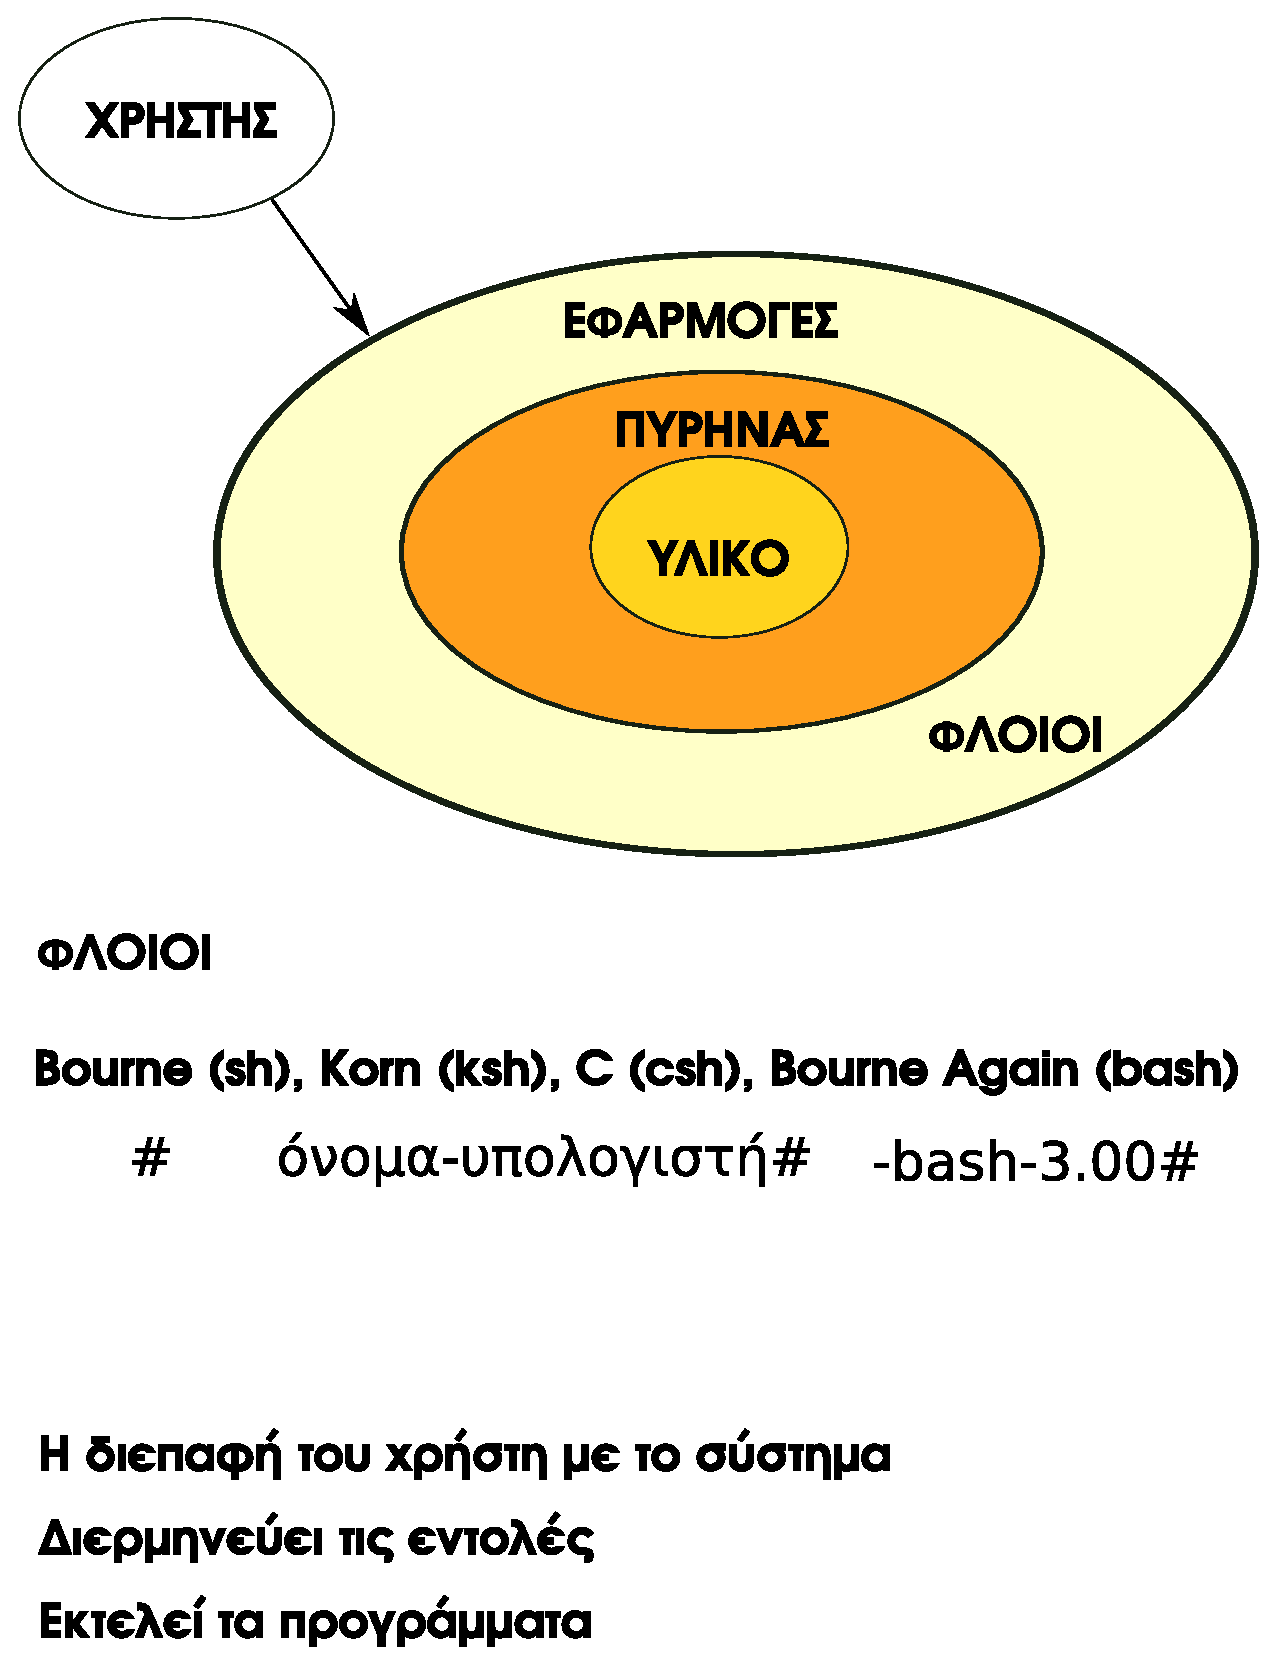
\includegraphics{shells.eps}}
	\scalebox{0.7}{\includegraphics[angle=90]{images/vim-cs.png}}
	\caption{vim cheetsheet \href{https://imgur.com/gallery/wjtaaxh}{https://imgur.com/gallery/wjtaaxh}}
\end{figure*} 


\begin{comment}
\section{Επεξεργασία Ρεύματος}

\subsection{awk}

Το όνομά του προέρχεται από τους Alfred \textbf{A}ho, Peter \textbf{W}einberger και Brian \textbf{K}ernighan και είναι μια γλώσσα προγραμματισμού σχεδιασμένη να εντοπίζει συγκεκριμένα πρότυπα και να εφαρμόζει σε αυτά κάποιες ενέργειες.  

Η λογική του awk είναι ότι εφαρμόζει ένα σύνολο από ενέργειες όταν βρεθεί ένα pattern.

 
\subsection{sed}
\end{comment}


%----------------------------------------------------------------------------------------


